\chapter{Interpolación polinómica}
\section{Introducción}
Una de las herramientas más potentes del análisis numérico es el teorema de Taylor, que nos permite aproximar el valor de una función en un punto por el valor de su polinomio de Taylor en dicho punto. Utilizar este tipo de desarrollo es útil cuando conocemos un único valor de dicha función. Sin embargo, el hecho de conocer el valor de la función en más de un punto nos permite desarrollar técnicas para calcular polinomios que aproximen la función de una forma más precisa. 

Además, la aproximación de una función por un polinomio es algo ampliamente utilizado a la hora de resolver problemas que pueden no tener solución analítica (derivada de la función en un punto, integrales definidas, ecuaciones diferenciales, etc.) y minimizando el error cometido al aproximar la función minimizaremos también el error de la aproximación realizada para solucionar el problema.

En primer lugar determinaremos las condiciones que debe cumplir un polinomio para que pase por un conjunto de puntos del plano y las fórmulas para calcularlo explícitamente (forma de Lagrange, fórmulas de Newton-Gregory, etc.). Trataremos también el problema de determinar los nodos para que el error de interpolación sea mínimo. La última parte del capítulo trata sobre la interpolación de Hermite, una técnica que se puede considerar la generalización del polinomio de Taylor.
        \section{Interpolación de Lagrange}
        
        \begin{defin}
        Dada $f: \mathbb{R} \longrightarrow \mathbb{R}$ y $\{x_o, \ldots, x_n\}$ diremos que $p_n(x) \in \mathbb{R}[x]$ de grado menor o igual que $n$ \textbf{interpola} a $f$ en esos puntos cuando 
        $$p_n(x_i)=f(x_i)=f_i \quad \forall i = 0, \ldots, n$$
        llamaremos \textbf{nodos} a los puntos $x_i$.
        \end{defin}
        \begin{ejes}\:
        \vspace{-3mm}
        \begin{itemize}
            \item Dado $x_0$, el polinomio de interpolación es $p_o(x)=f(x_0)$ (recta horizontal que pasa por $f(x_o)$).
            \item Dados $x_0,x_1$, el polinomio de interpolación para $n=2$ será $p_1(x)=f(x_0)\cdot \frac{x-x_0}{x_1-x_0}+f(x_1)\cdot \frac{x-x_1}{x_0-x_1}$ (recta que une los puntos $f(x_o)$ y $f(x_1)$).
            
        \end{itemize}
        \end{ejes}
        
        \begin{teo}
        
        Dada $f: \mathbb{R} \longrightarrow \mathbb{R}$ y los $n+1$ puntos distintos $\{x_o, \ldots, x_n\}$, existe un {\'u}nico polinomio $p_n(x)$ de grado menor o igual que $n$ que interpola a $f$ en los puntos dados.
        \end{teo}
        
        \begin{dem}
        
        Denotemos por $\mathbb{P}_n[x]$ al $\mathbb{R}-$espacio vectorial de polinomios de grado menor o igual que $n$, que será de dimensi{\'o}n $n+1$. Definimos:
        $$\begin{array}{rrcl}
            \psi : & \mathbb{P}_n[x] & \longrightarrow & \mathbb{R}^{n+1} \\
            \: & p(x) & \longmapsto & \psi(p(x))=(p(x_o), \ldots, p(x_n)) 
        \end{array}$$
        donde $\psi$ es una aplicaci{\'o}n trivialmente lineal. Si $p(x) \in Ker \: \psi$, se tiene que
        $$\psi(p(x))=(p(x_o), \ldots, p(x_n)) = (0, \ldots, 0)$$
        que es equivalente a  $p(x_i)=0 \; \forall i \in \{0, \ldots, n\}$. Como $gr(p_n) \leq n$ y tiene $n+1$ ra{\'i}ces necesariamente $p(x)=0$. Por tanto, $\psi$ es inyectiva y epiyectiva (por c{\'o}mputo de dimensiones), luego $\psi$ isomorfismo. 
        
        Con esto podemos concluir que la solución al problema de interpolación existe y es única, siendo dicha solución $\psi^{-1}(f(x_0),\ldots,f(x_n))$.
        \qed\end{dem}
        \begin{cor}
        Las formas lineales $\omega_i:\mathbb{P}_n[x]\rightarrow\mathbb{R}$ dadas por $\omega_i(p(x))=p(x_i)$ forman una base de $\mathbb{P}^*_n[x]$. Su base dual son los polinomios $\{\ell_i(x)\}_{i=0}^n$ (denominados \textbf{polinomios de Lagrange}) dados por la expresión
        \begin{align}
         \ell_i(x)=\prod_{i \neq j} \dfrac{(x-x_i)}{(x_i-x_j)}   
         \label{pol:lag}
        \end{align}
        y por definición de base dual sabemos que podemos expresar cualquier polinomio $p(x)$ de la siguiente forma:
        $$p(x)=\sum_{i=0}^n \omega_i(p_n(x))\cdot  \ell_i(x)$$
        Con lo cual, el polinomio de interpolación de la función $f$ en los puntos $\{x_o,x_1,\ldots,x_n\}$ es
        \begin{align}
        p_n(x)=\sum_{i=0}^n \omega_i(p_n(x))\cdot  \ell_i(x)=\sum_{i=0}^n p_n(x_i)\cdot  \ell_i(x)=\sum_{i=0}^n f(x_i)\cdot  \ell_i(x)
        \label{pol:lagrange}
        \end{align}
        este es el \textbf{polinomio de interpolación de Lagrange}.
        \end{cor}
        \begin{obs}
        El problema de interpolar una función se puede resolver para cualquier base del espacio $\mathbb{P}_n[x]$.  Consideremos la base $\{1, x,\ldots, x^n\}$. Debemos encontrar $a_0,\ldots,a_n\in\mathbb{R}$ tales que
        $$a_nx_i^n+\ldots+a_1x_i+a_o=f(x_i)\qquad i=0,\ldots, n$$
        Lo cual es un sistema de $n+1$ ecuaciones con $n+1$ incógnitas cuya representación matricial es
        $$
        \left(\begin{array}{ccccc}
            1 &x_o&x_o^2&\cdots &x_o^n  \\
            1 &x_1&x_1^2&\cdots &x_1^n \\
            \vdots &\vdots&\vdots&\ddots &\vdots\\
            1 &x_n&x_n^2&\cdots &x_n^n
        \end{array}\right)\left(\begin{array}{c}
             a_o  \\
             a_1\\
             \vdots\\
             a_n
        \end{array}\right)=\left(\begin{array}{c}
             f(x_o)  \\
             f(x_1)\\
             \vdots\\
             f(x_n)
        \end{array}\right)
        $$
        donde la primera matriz es la \textbf{matriz de Vandermonde}, que será invertible siempre y cuando los $x_i$ sean distintos, esto es, el sistema será compatible determinado siempre y cuando los $x_i$ sean distintos. 
        
        Este método de interpolación no es el más aconsejable dado que la matriz de Vandermonde está mal condicionada (pequeños cambios en los $x_i$ cambian significativamente los valores de los $a_i$).
        \end{obs}
        \section{Interpolación de Newton}
        \begin{teo}
         Dados $n+1$ puntos distintos $\{x_o,\ldots,x_n\}$, los polinomios $\{1,(x-x_o),\ldots,(x-x_o)\cdot\ldots\cdot(x-x_{n-1})\}$ forman una base de $\mathbb{P}_n[x]$.
        \end{teo}
        \begin{dem}
       Dada una combinación lineal arbitraria de dichos polinomios igualada a cero, se tiene que
       $$\lambda_o+\lambda_1 (x-x_o)+\ldots+\lambda_n (x-x_o)\cdot\ldots\cdot(x-x_{n-1})=0$$
       $$\lambda_o+\lambda_1 (x-x_o)+\ldots+\lambda_{n-1}(x-x_o)\cdot\ldots\cdot(x-x_{n-2})=-\lambda_n (x-x_o)\cdot\ldots\cdot(x-x_{n-1})$$
      Como el polinomio del miembro izquierdo es de grado $n-1$ y el del derecho es de grado $n$, necesariamente ambos son nulos y, por tanto, $\lambda_i=0$ para todo $i=0,\ldots,n$. Con lo cual los polinomios considerados son linealmente independientes (luego base).
        \qed\end{dem}
        \begin{cor}
        Podemos concluir entonces que dados $n+1$ puntos distintos $\{x_o,\ldots,x_n\}$ todo polinomio $p(x)$ se puede expresar de la siguiente forma:
        $$p(x)=\sum_{i=0}^n c_i\cdot (x-x_o)\cdot\ldots\cdot(x-x_{i-1})$$
        De esta forma, el polinomio de interpolación $p_n$ de los puntos $\{x_o,\ldots,x_n\}$  lo podemos expresar como sigue
        $$p_n(x)=\sum_{i=0}^n c_i\cdot (x-x_o)\cdot\ldots\cdot(x-x_{i-1})=\sum_{i=0}^{n-1} c_i\cdot (x-x_o)\cdot\ldots\cdot(x-x_{i-1})+c_n\cdot(x-x_o)\cdot\ldots\cdot(x-x_{n-1})=$$
        \begin{align}
        =p_{n-1}(x)+c_n\cdot (x-x_o)\cdot\ldots\cdot(x-x_{n-1})
        \label{ec:newton}
        \end{align}
        este es el \textbf{polinomio de interpolación de Newton}.
        
        \end{cor}
        \begin{obs}
        La forma más óptima de computar este polinomio es con la denominada \textbf{multiplicación anidada de Horner}:
        $$p_n(x)=c_o+c_1(x-x_o)+c_2(x-x_o)(x-x_1)+\ldots+c_n(x-x_o)\ldots(x-x_{n-1})=$$
        $$=c_o+(x-x_o)[c_1+c_2(x-x_1)+\ldots+c_n(x-x_1)\ldots(x-x_{n-1})]=$$
        $$=c_o+(x-x_o)[c_1+(x-x_1)[c_2+\ldots+(x-x_{n-2})[c_{n-1}+c_n(x-x_{n-1})]\cdots]$$
        de forma que para $n=2$ tenemos la siguiente expresión para el polinomio de interpolación:
        $$p_2(x)=c_o+(x-x_o)[c_1+(x-x_1)c_2]$$
        
        \end{obs}
        \begin{cor}
        Si tomamos $x=x_n$ en (\ref{ec:newton}) podemos obtener una expresión para calcular el coeficiente $c_n$:
        $$f(x_n)=p_n(x_n)=p_{n-1}(x_n)+c_n(x_n-x_o)\cdots(x_n-x_{n-1})\Longrightarrow c_n=\frac{f(x_n)-p_{n-1}(x_n)}{\prod_{i=0}^{n-1}(x_n-x_i)}$$
        Sin embargo, esta no es la forma más eficiente de calcular estos coeficientes. Por ello introduciremos a continuación la noción de diferencia divididas.
        
        \end{cor}

        \section{Diferencias divididas}
        \begin{defin}
        Dados $n+1$ puntos distintos $\{x_o,\ldots,x_n\}$, se define la diferencia dividida de una función $f$ en $x_o$ como
        $$f[x_o]=f(x_o)$$
        y la diferencia dividida primera de $f$ en $x_o,x_1$ 
        $$f[x_o,x_1]=\frac{f[x_1]-f[x_o]}{x_1-x_o}=\frac{f(x_1)-f(x_o)}{x_1-x_o}$$
        Se define entonces la \textbf{diferencia dividida n-ésima} en $x_o,\ldots,x_n$ como
        \begin{align}
        f[x_o,\ldots,x_n]=\frac{f[x_1,\ldots,x_n]-f[x_o,\ldots,x_{n-1}]}{x_n-x_o} 
        \label{dif:div}
        \end{align}
        \end{defin}
        \begin{prop}
         Sean $n+1$ puntos distintos $\{x_o,\ldots,x_n\}$ y $p_n(x),p_{n-1}(x)$ los polinomios de interpolación de $f$ en $\{x_o,\ldots,x_n\}$ y $\{x_o,\ldots,x_{n-1}\}$ respectivamente. Entonces
         $$p_n(x)=p_{n-1}(x)+c_n(x-x_o)\ldots(x-x_{n-1})$$
         donde
         $$c_n=f[x_o,\ldots,x_n]$$
        \end{prop}
        \begin{dem}
        Por inducción sobre $n$. Para $n=1$ se tiene que
        $$p_1(x)=p_o(x)+c_1(x-x_o)=f(x_o)+c_1(x-x_o)$$
        tomando $x=x_1$ podemos concluir que
        $$c_1=\frac{p_1(x_1)-f(x_o)}{x_1-x_o}=\frac{f(x_1)-f(x_o)}{x_1-x_o}=f[x_o,x_1]$$
       Sea $q_{n-1}$ el polinomio de interpolación de $f$ en $\{x_1,\ldots,x_n\}$. Supongamos que para cierto $n\geq1$ se verifica que:
       $$p_{n-1}(x)=p_{n-2}(x)+f[x_o,\ldots,x_{n-1}](x-x_o)\ldots(x-x_{n-2})$$
       $$q_{n-1}(x)=q_{n-2}(x)+f[x_1,\ldots,x_n](x-x_1)\ldots(x-x_{n-1})$$
        Consideremos el siguiente polinomio:
        $$R_n(x)=p_{n-1}(x)\cdot\frac{x-x_n}{x_o-x_n}+q_{n-1}(x)\cdot\frac{x-x_o}{x_n-x_o}$$
        Si tomamos $x=x_o$:
        $$R_n(x_o)=p_{n-1}(x_o)\cdot\frac{x_o-x_n}{x_o-x_n}+q_{n-1}(x)\cdot\frac{x_o-x_o}{x_n-x_o}=p_{n-1}(x_o)=f(x_o)$$
        y si tomamos $x=x_n$
        $$R_n(x_o)=q_{n-1}(x_n)=f(x_n)$$
        Finalmente, tomando $x=x_i$ ($0<i<n$):
        $$R_n(x_i)=p_{n-1}(x_i)\cdot\frac{x_i-x_n}{x_o-x_n}+q_{n-1}(x_i)\cdot \frac{x_i-x_o}{x_n-x_o}=\frac{f(x_i)}{x_n-x_o}\cdot(x_i-x_o-(x_i-x_n))=f(x_i)$$
        Luego $R_n(x)$ interpola a $f$ en todos los $x_i$ y por tanto, debe ser el polinomio de interpolación, esto es:
        $$p_n(x)=p_{n-1}(x)\cdot\frac{x-x_n}{x_o-x_n}+q_{n-1}(x)\cdot\frac{x-x_o}{x_n-x_o}$$
        Por definición, $c_n$ es el coeficiente de grado $n$ de $p_n(x)$. Comparándolo con el coeficiente de mayor grado del miembro derecho podemos concluir que:
        $$c_n=\frac{f[x_o,\ldots,x_{n-1}]}{x_o-x_n}+\frac{f[x_1,\ldots,x_n]}{x_n-x_o}=\frac{f[x_1,\ldots,x_n]-f[x_o,\ldots,x_{n-1}]}{x_n-x_o}=f[x_o,\ldots,x_n]$$
        \qed\end{dem}
        \begin{cor}
        Las diferencias divididas son invariantes por permutaciones:
        $$f[x_o,\ldots,x_ n]=f[x_{\sigma(o)},\ldots,x_{\sigma(n)}]\qquad \forall\sigma\in S_{n+1}$$
        Esto es debido a la unicidad el polinomio de interpolación
        \end{cor}
        
        \section{Error de interpolación}
        \begin{prop}
        Sea $f$ una función $n$ veces derivable en un intervalo $I$ y $\{x_o,\ldots,x_n\}$ $n+1$ puntos distintos de $I$. Entonces, existe un punto $\xi\in I$ tal que
        $$f[x_o,\ldots,x_n]=\frac{f^{(n)}(\xi)}{n!}$$
        para $n=1$ tenemos el Teorema de los Incrementos Finitos (o Teorema del Valor Medio).
        \end{prop}
        \begin{dem}
        Sea $p_n(x)$ el polinomio de interpolación de $f$ en $\{x_o,\ldots,x_n\}$ y sea $\phi_n(x)=f(x)-p_n(x)$. Por definición del polinomio de interpolación, sabemos que $\phi(x_i)=0$ para cualquier $i=0,\ldots,n$.
        
        Por el Teorema de Rolle, sabemos que $\phi'_n(\xi^{(1)}_i)=0$ para ciertos $\xi^{(1)}_i\in(x_{i-1},x_i)$ con $i=1,\ldots,n$. De nuevo por el Teorema de Rolle podemos afirmar que existen $\xi_i^{(2)}\in(\xi_{i-1}^{(1)},\xi_i^{(1)})$ tales que $\phi_n''(\xi_i^{(2)})=0$ con $i=2,\ldots n$. Reiterando este proceso, podemos concluir que existe $\xi^{(n)}_n=\xi$ tal que $\phi^{(n)}_n(\xi^{(n)}_n)=0$. Ahora bien, $$\phi^{(n)}_n(\xi)=f^{(n)}(\xi)-p^{(n)}_n(\xi)=f^{(n)}(\xi)-f[x_o,\ldots,x_n]\cdot n!=0$$
        y por tanto 
       $$f[x_o,\ldots,x_n]=\frac{f^{(n)}(\xi)}{n!}$$

        \qed\end{dem}
        \begin{teo}
         Sea $f$ una función $n$ veces derivable en un intervalo $I$ y $\{x_o,\ldots,x_n\}$ $n+1$ puntos distintos de $I$. Si $p_n(x)$ es el polinomio de interpolación de $f$ en dichos puntos, entonces para todo $x\in I$ tenemos que
         \begin{align}
         \mathcal{E}_n(x)=f(x)-p_n(x)=\frac{f^{(n+1)}(\xi)}{(n+1)!}(x-x_o)\cdots(x-x_n)
         \label{error:int}
          \end{align}
        \end{teo}
        \begin{dem}
        Si $x=x_i$ para algún $i=0,\ldots, n$ la fórmula es cierta (ambos lados de la igualdad se anulan). Supongamos entonces que $x\neq x_i$ y sea entonces $p_{n+1}$ el polinomio de interpolación de $f$ en $\{x_o,\ldots,x_n,x\}$. Se tiene entonces que:
        $$\mathcal{E}_n=f(x)-p_n(x)=p_{n+1}(x)-p_n(x)=f[x_o,\ldots,x_n,x](x-x_o)\cdots(x-x_n)$$
        donde hemos usado la fórmula de Newton para el polinomio de interpolación. Usando ahora la proposición anterior, se deduce que
        $$\mathcal{E}_n(x)=f(x)-p_n(x)=\frac{f^{(n+1)}(\xi)}{(n+1)!}(x-x_o)\cdots(x-x_n)$$
        con $\xi\in I$.
        \qed\end{dem}
        \begin{obs}
        La fórmula obtenida para el error de interpolación es parecida a la expresión del error de la fórmula de Taylor. El hecho de que aparezca el término $(n+1)!$ en el denominador parece indicar que el error tiende a 0 a medida que aumenta la $n$ (al igual que en la fórmula de Taylor). Sin embargo, esto no es así. Para ciertas funciones, el error de interpolación no disminuye al considerar cada vez más nodos, lo cual se conoce como \textbf{fenómeno de Runge}.
        
        Consideremos la función $f(x)=\frac{1}{25x^2+1}$. En la Figura \ref{fig:runge} se ha representado dicha función en el intervalo $[-1,1]$ (en azul) junto con los polinomios de interpolación de grado $10$ (en rojo) y de grado $15$ (en verde), tomando nodos uniformemente distribuidos. Se puede apreciar cómo el polinomio de interpolación va oscilando de forma cada vez más abrupta en los extremos a medida que aumenta el número de nodos.. Esto nos indica que el error de interpolación (máximo) no tiende a $0$ sino que crece infinitamente. \label{runge }
        \begin{figure}[h]
            \centering
            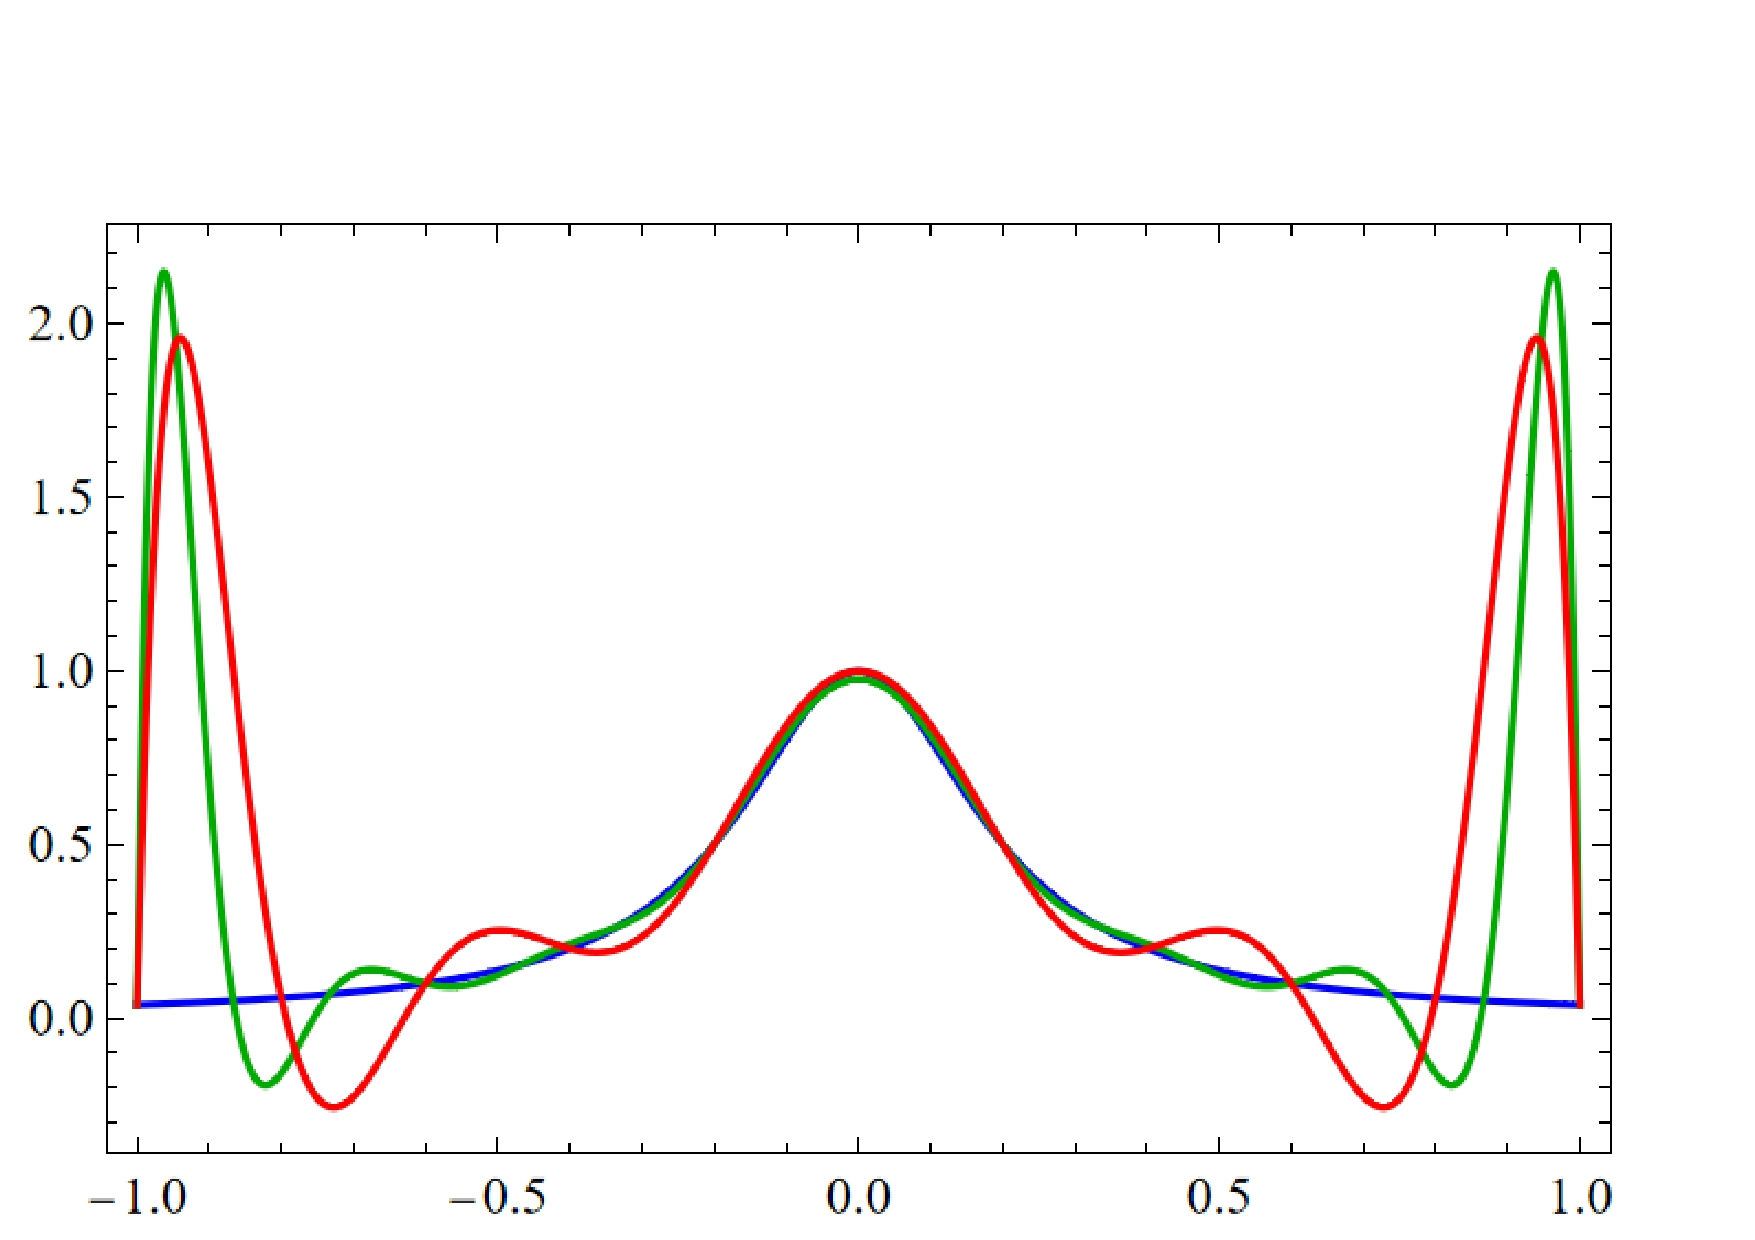
\includegraphics[scale=0.5]{runge3_page-0001.jpg}
            \caption{Fenómeno de Runge}
            \label{fig:runge}
        \end{figure}
    
        \end{obs}
        \begin{cor}
        Si analizamos el máximo del error de interpolación en todo el intervalo $I$ tenemos que
        $$\underset{x\in I}{\max}|f(x)-p_n(x)|=\|f(x)-p_n(x)\|_{\infty,I}=\left\|\frac{f^{(n+1)}(\xi)}{(n+1)!}\cdot \omega_n\right\|_{\infty,I}$$
        donde $\omega_n=(x-x_o)\cdots(x-x_n)$. De esta forma
        $$\underset{x\in I}{\max}|f(x)-p_n(x)|\leq \frac{\|f^{(n+1)}\|_{\infty,I}}{(n+1)!}\cdot \|\omega_n\|_{\infty,I}$$
        La forma de reducir este error es usando los nodos de Chebysev, que serán aquellos puntos que minimicen la función $\|\omega_n\|_{\infty}$.
        \end{cor}
        
        \section{Nodos de Chebyshev}
        \begin{defin}
        Fijemos el intervalo $I=[-1,1]$. Se definen los \textbf{polinomios de Chebyshev} (denotados por $T_n(x)$) por la siguiente fórmula de recurrencia:
        $$T_o(x)=1$$
        $$T_1(x)=x$$
        \begin{align}
        T_{n+1}(x)=2x\cdot T_{n}(x)-T_{n-1}(x)   
        \label{pol:cheb}
        \end{align}
        En la Figura \ref{fig:chebyshev} se han representado los primeros  $7$ polinomios de Chebyshev.
                 \begin{figure}[h]
            \centering
            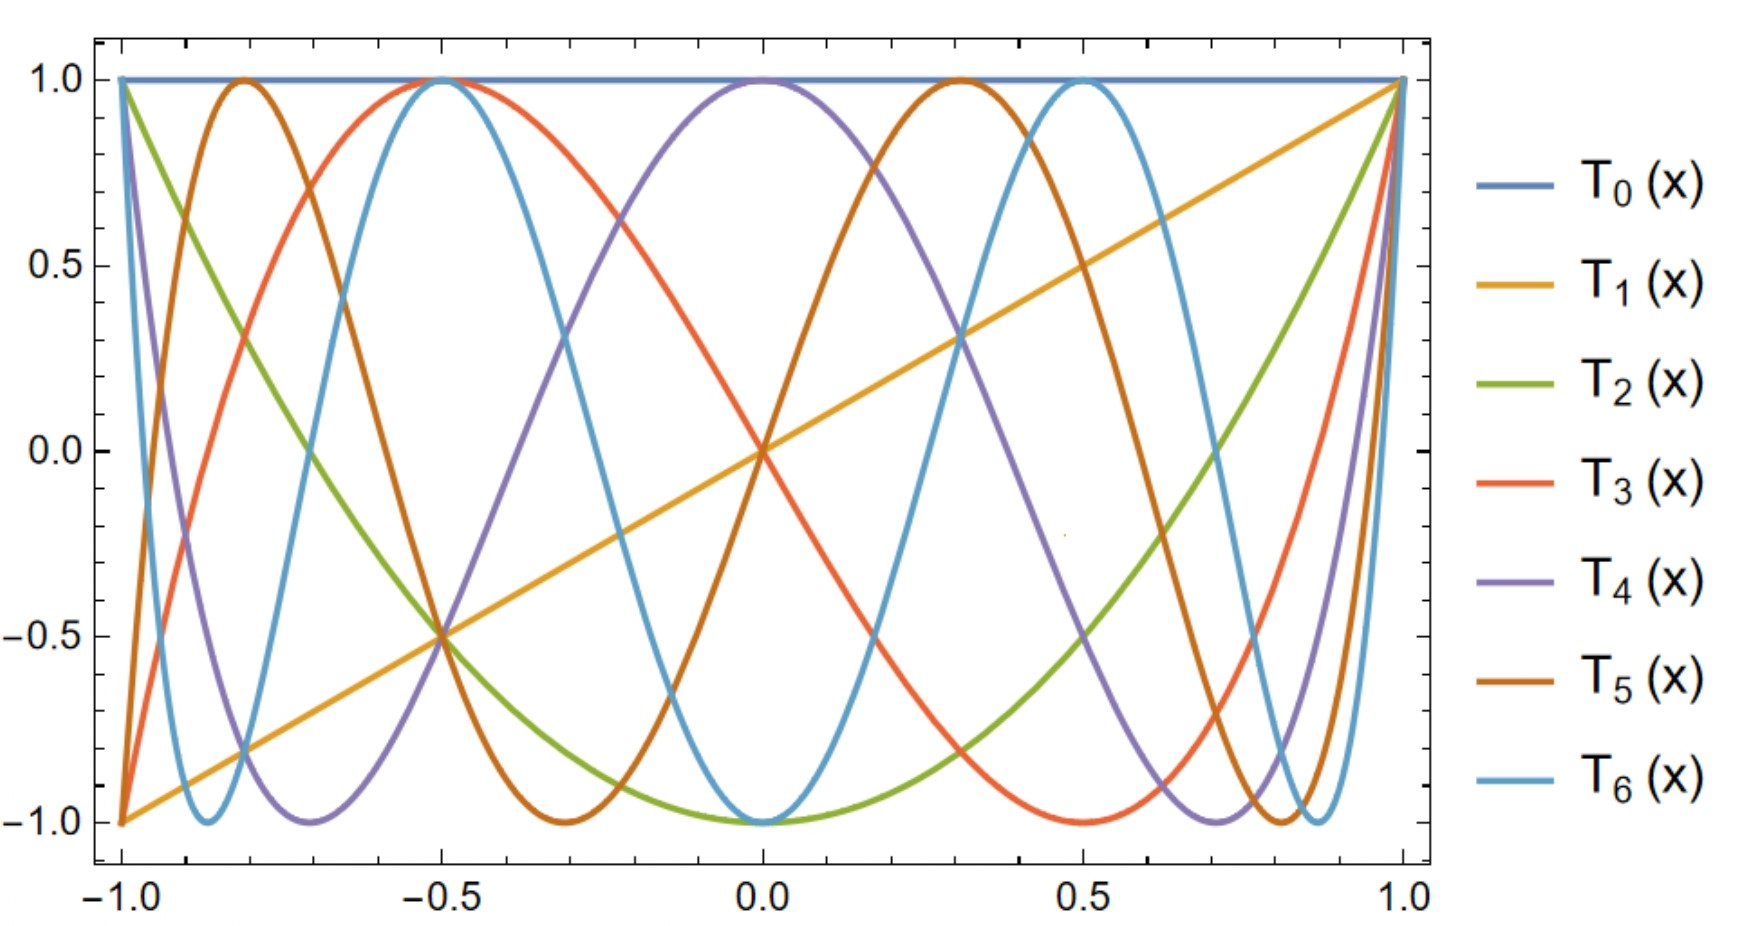
\includegraphics[scale=0.5]{chebyshev_page-0001.jpg}
            \caption{Polinomios de Chebyshev}
            \label{fig:chebyshev}
        \end{figure}
        
        \end{defin}
       
        \begin{prop}
        Para todo $x\in[-1,1]$ se verifica que
        $$T_n(\cos \theta)=\cos(n\theta)$$ o, equivalentemente, que $$T_n(x)=\cos(n\cdot \arccos(x))$$ 
        \end{prop}
        \begin{dem}
        Haremos la demostración por inducción sobre $n$. Para $n=0$ se tiene trivialmente que $1=T_o(\cos\theta)=\cos(0\cdot \theta)$.
        Supongamos que la fórmula es cierta para cierto $n\geq 0$, entonces:
        $$T_{n+1}(\cos\theta)=2\cos\theta\cdot T_n(\cos\theta)-T_{n-1}(\cos\theta)=2\cos\theta\cdot \cos(n\theta)-\cos((n-1)\theta)=$$
        $$=2\cos\theta\cdot\cos(n\theta)-(\cos(n\theta)\cdot \cos(-\theta)-\sin(n\theta)\cdot \sin(-\theta))$$
        $$=2\cos\theta\cdot\cos(n\theta)-\cos(n\theta)\cdot \cos(\theta)+\sin(n\theta)\cdot \sin(\theta))= \cos((n+1)\theta)$$
        como queríamos demostrar.
        \qed\end{dem}

        \begin{cor}\:\vspace{-5mm}
        \begin{itemize}
            \item[a)] $T_n(-x)=(-1)^n\cdot T_n(x)$
            \item[b)] El coeficiente de grado máxmo de $T_n$ es $2^{n-1}$ para $n\geq1$
            \item[c)] $\|T_n\|_{\infty,I}=1$
            \item[d)] $T_n$ tiene $n+1$ extremos en $I$.
            \item[e)] $T_n$ tiene todas sus raíces en $I$ y son distintas
        \end{itemize}
        \end{cor}

        \begin{dem}\:\vspace{-5mm}
        \begin{itemize}
            \item[a)] Por inducción sobre $n$. El caso $n=0$ es obvio. Supongamos que es cierto para algún $n\geq0$, entonces:
            $$T_{n+1}(-x)=2(-x)\cdot T_n(-x)-T_{n-1}(-x)=2(-x)\cdot (-1)^n\cdot T_n(x)-(-1)^{n-1}T_{n-1}(x)=$$
            $$=(-1)^{n-1}(2x\cdot T_n(x)-T_{n-1}(x))=(-1)^{n+1}T_{n+1}(x)$$
            \item[b)] De nuevo por inducción sobre $n$. Para $n=1$ es cierto por ser el coeficiente de mayor grado $1=2^0$. Supongamos que para cierto $n\geq 1$ se verifica que el coeficiente de mayor grado de $T_n$ es $2^{n-1}$, es decir, que $$T_{n}=2^{n-1}x^n+r_1(x)$$
            donde $r_1(x)$ denota los términos de grado menor que $n$. Se tiene entonces que
            $$T_{n+1}=2x\cdot T_n-T_{n-1}=2^nx^{n+1}+r_2(x)+T_{n-1}(x)$$
            como los grados de $r_2(x)=2x\cdot r_1(x)$ y $T_{n-1}(x)$ son menores o iguales que $n$, el coeficiente de mayor grado de $T_{n+1}$ es $2^n$ como queríamos demostrar.
            \item[c)] Como $T_n(\cos\theta)=\cos(n\theta)$ se tiene que
            $$\|T_n(\cos\theta)\|_{\infty,I}=\|\cos(n\theta)\|_{\infty,I}\leq 1$$
            \item[d)] Sabemos que $\underset{x\in I}{\max}|T_n(x)|=1$, luego basta con encontrar los $x\in I$ que verifiquen $T_n(x)=\pm 1$:
            $$T_n(x)=T_n(\cos\theta)=\cos(n\theta)=\pm1$$
            y esto solo ocurre cuando $n\theta=k\pi$ con $k\in\mathbb{Z}$, es decir, $\theta=k\cdot\frac{\pi}{n}$. Podemos decir entonces que $T_n(x'_k)=\pm 1$ cuando $x'_k=\cos\left(k\cdot\frac{\pi}{n}\right)$, $k=0,\ldots,n$, que serán $n+1$ puntos como queríamos demostrar. Además:
            $$T_n(x_{k+1})=\cos\left(\frac{\pi}{2}(2(k+1)+1)\right)=\cos\left(k\pi +\frac{3\pi}{2}\right)=\cos(k\pi)$$
            $$T_n(x_k)=\cos\left(\frac{\pi}{2}(2k+1)\right)=\cos\left(k\pi+\frac{\pi}{2}\right)=-\cos(k\pi)$$
            luego $T_n(x'_{k+1})=-T_n(x'_k)$.
            \item[e)] Como hemos visto, en el intervalo $[x'_{k+1},x'_{k}]$ se verifica que $T_n(x'_{k+1})=-T_n(x'_k)$. Aplicando el Teorema de Bolzano, $T_n(x)$ tiene una raíz en cada intervalo $[x'_{k+1},x'_{k}]$. En total habrá $n$ raíces y como $T_n(x)$ es de grado $n$, serán todas.

            Estas raíces las podemos calcular resolviendo la ecuación
            $$T_n(\cos\theta)=\cos(n\theta)=0\Longleftrightarrow n\theta=\frac{\pi}{2}+k\pi\qquad k\in\mathbb{Z}$$
            con lo cual, $\theta=\frac{\pi}{2n}(2k+1)$ con $k\in\mathbb{Z}$ y las raíces de los polinomios de Chebyshev serán entonces
            $$x_k=\cos\left(\frac{\pi}{2n}(2k+1)\right)\qquad k\in \mathbb{Z}$$
        \end{itemize}
        \qed\end{dem}
        \begin{defin}
        Denominaremos \textbf{nodos de Chebyshev} a las raíces de los polinomios de Chebyshev. Como acabamos de demostrar, en el intervalo $[-1,1]$ vienen dados por la expresión:
        \begin{align}
        x_k=\cos\left(\frac{\pi}{2n}(2k+1)\right)\qquad k\in \mathbb{Z}
        \label{nodos:cheb}
        \end{align}
        \end{defin}
        \begin{teo}
        El polinomio de Chebysev $T_n(x)$ es el polinomio con la norma infinto mínima en el intervalo $[-1,1]$ entre todos los polinomios de grado $n$ y coeficiente de grado máximo $2^{n-1}$. En otras palabras, si denotamos por $T_n'(x)=\frac{1}{2^{n-1}}T_n(x)$ entonces
        $$\|T_n'\|_{\infty,I}<\|p_n\|_{\infty,I}$$
        donde $p_n$ es cualquier polinomio de grado $n$ y mónico.
        \end{teo}
        \begin{dem}
        Sea $p_n(x)$ un polinomio mónico de grado $n$ tal que
        $$\|p_n\|_{\infty,I}\leq\|T_n'\|_{\infty,I}$$
        Por el corolario anterior, $T'_n(x)$ tiene sus extremos en los puntos $x'_k=\cos\left(k\cdot\frac{\pi}{n}\right)$ y, por tanto
        $$T'_n(x'_k)=\frac{\pm 1}{2^{n-1}}$$
        Observemos entonces que
        $$\frac{1}{2^{n-1}}=T'_n(x'_o)>p_n(x'_o)$$
        $$\frac{-1}{2^{n-1}}=T'_n(x'_1)<p_n(x'_1)$$
        $$\frac{1}{2^{n-1}}=T'_n(x'_2)>p_n(x'_2)$$
        $$\vdots$$
        En cualquier caso, el polinomio  diferencia $T'_n-p_n$ tiene signo contrario en los extremos de cada uno de los intervalos $[x'_{k+1},x'_k]$. Aplicando el Teorema de Bolzano podemos concluir que $T'_n-p_n$ tiene una raíz en cada intervalo, esto es, tiene $n$ raíces. Sin embargo, $T'_n-p_n$ es de grado $n-1$ ya que ambos son polinomios mónicos, lo cual no es posible y por tanto, no existe el polinomio $p_n(x)$.
        \qed\end{dem}
        \begin{cor}
        Sea $p_n$ el polinomio de interpolación de $f$ en los nodos de Chebysev $\{x_o,\ldots,x_n\}$. Para cada $x\in[-1,1]$ se tiene que
        $$|f(x)-p_n(x)|\leq\frac{\|f^{(n+1)}\|_{\infty,I}}{(n+1)!}\left\|\prod_{k=0}^n(x-x_k)\right\|_{\infty,I}$$
    el productorio del miembro derecho es precisamente el polinomio de Chebysev de grado $n$ multiplicado por un factor de $\frac{1}{2^{n-1}}$, con lo cual:
    $$|f(x)-p_n(x)|\leq \frac{\|f^{(n+1)}\|_{\infty,I}}{2^{n-1}(n+1)!}$$
        \end{cor}
        \begin{ejem}

        Siguiendo el ejemplo de la \textit{Observación} (pág. 23), calculemos el polinomio de interpolación de grado $15$ de la función $f(x)=\frac{1}{25x^2+1}$ utilizando los nodos de Chebyshev. El resultado se expone en la Figura \ref{fig:chebyshev2}, donde se puede apreciar que el fenómeno de Runge se ha reducido al mínimo.
        \begin{figure}[h]
            \centering
            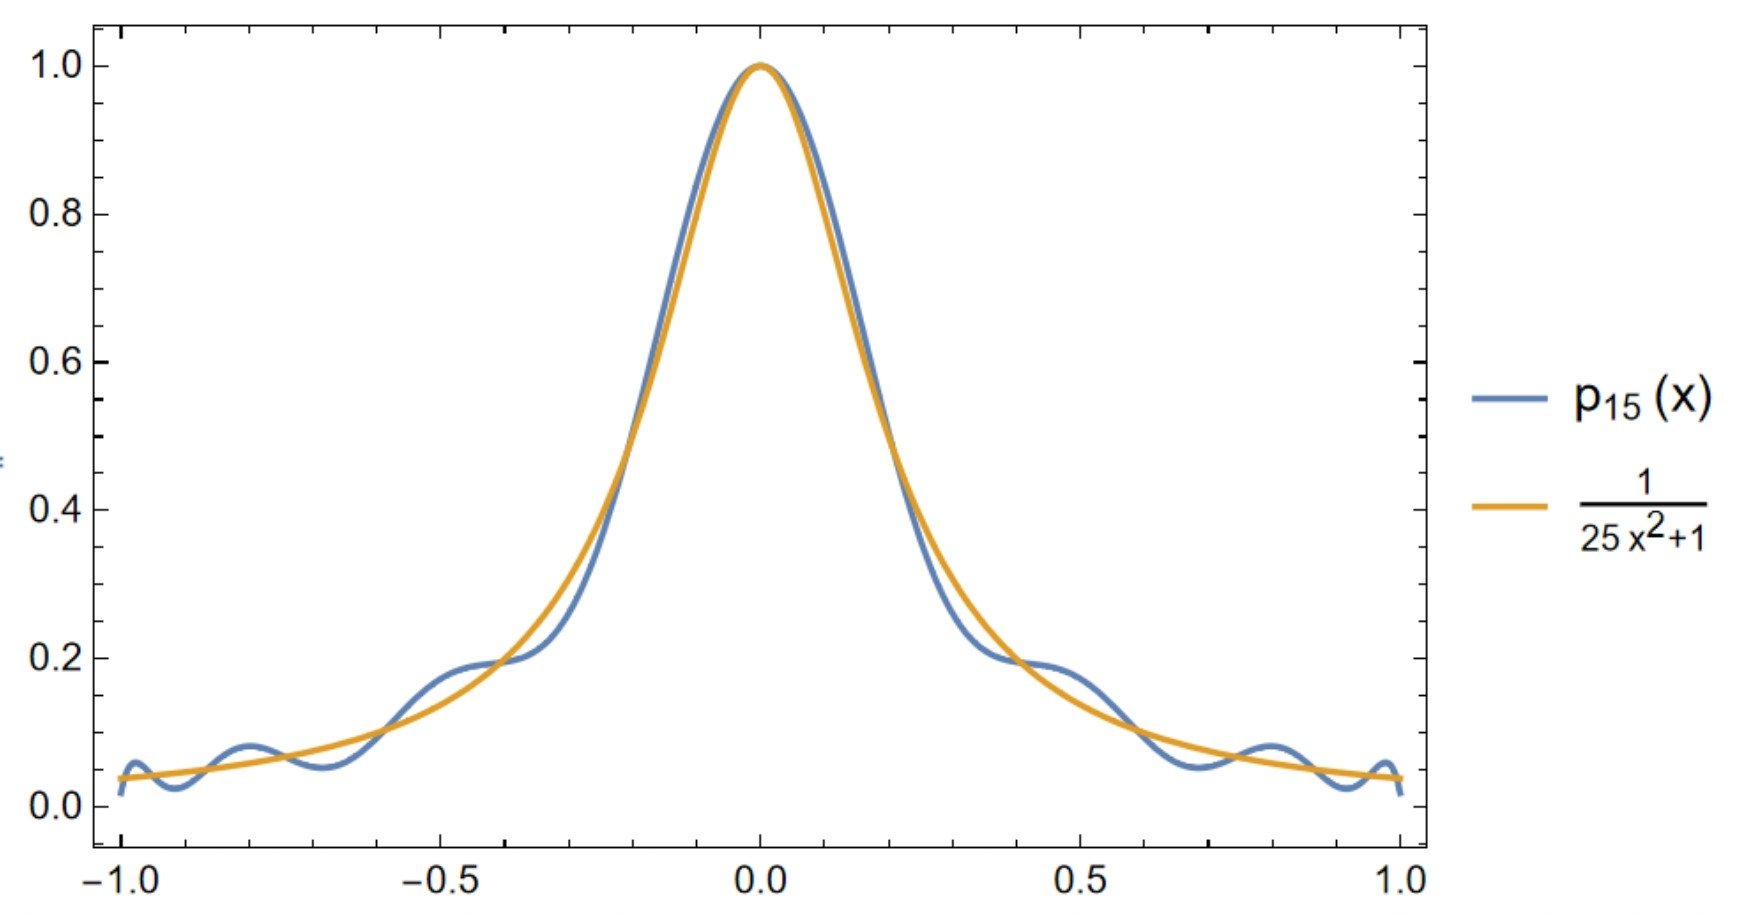
\includegraphics[scale=0.5]{chebyshev2_page-0001 (1).jpg}
            \caption{Polinomio de interpolación utilizando los nodos de Chebyshev}
            \label{fig:chebyshev2}
        \end{figure}
        \end{ejem}
        \begin{obs}
        El estudio que hemos realizado sobre los nodos de Chebyshev en el intervalo $[-1,1]$ es también válido para cualquier intervalo de la recta real. Dado el intervalo $[a,b]$, hacemos el cambio de variable
        $$\psi(t)=\frac{a+b}{2}+t\frac{b-a}{2}\qquad t\in [-1,1]$$
        para transformar el intervalo $[-1,1]$ en el intervalo $[a,b]$. Por tanto, dada una función cualquiera $f:[a,b]\longrightarrow \mathbb{R}$ podemos definir la función $f\circ\psi=\psi^*f:[-1,1]\longrightarrow\mathbb{R}$ .

        De esta manera, $\|f\|_{\infty,I}=\|\psi^*f\|_{\infty,I}$. Sean entonces $t_o,\ldots,t_n$ los nodos de Chebysev en $[-1,1]$ y $x_o,\ldots,x_n$ sus transformados por $\psi$, $x_k=\psi(t_k)$. Si $p_n$ es el polinomio de interpolación de $f$ en $\{x_0,\ldots,x_n\}$ se tiene que
        $$|f(x)-p_n(x)|\leq\frac{\|f^{(n+1)}\|_{\infty,I}}{(n+1)!}\left\|\prod_{k=0}^n(x-x_k)\right\|_{\infty,I}=$$
        $$=\frac{\|f^{(n+1)}\|_{\infty,I}}{(n+1)!}\left\|\prod_{k=0}^n\left(\frac{a+b}{2}+t\frac{b-a}{2}\right)-\left(\frac{a+b}{2}+t_k\frac{b-a}{2}\right)\right\|_{\infty,I}=\frac{\|f^{(n+1)}\|_{\infty,I}}{(n+1)!}\left\|\prod_{k=0}^n(t-t_k)\left(\frac{b-a}{2}\right)\right\|_{\infty,I}\leq$$
        $$\leq \frac{\|f^{(n+1)}\|_{\infty,I}}{(n+1)!}\cdot\frac{(b-a)^{n+1}}{2^{2n}}$$
        \end{obs}
        \section{Fórmulas de Newton-Gregory}
        \begin{defin}
        Dada una colección de nodos $\{x_o,\ldots,x_n\}$ diremos que están \textbf{equiespaciados o equidistantes} si $x_{i+1}=x_i +h$ para cierto $h>0$.
        \end{defin}
        \begin{defin}
        Sean $\{x_o,\ldots,x_n\}$ $n+1$ puntos distintos y $f:\mathbb{R}\longrightarrow\mathbb{R}$. Denominaremos \textbf{operador diferencia progresiva} al siguiente operador:
        $$\Delta f(x_i)=f(x_{i+1})-f(x_i)$$
        Equivalentemente, se define el \textbf{operador diferencia regresiva} como sigue
        $$\nabla f(x_i)=f(x_i)-f(x_{i-1})$$
        \end{defin}
        \begin{prop}
        Para todo $n\geq1$ se verifica que
        $$\Delta^n f(x_o)=\nabla ^n f(x_n)=\sum_{k=0}^n \binom{n}{k} (-1)^k f(x_{n-k})$$
        \end{prop}
        \begin{dem}
        Demostraremos la fórmula para el operador diferencia progresiva por inducción sobre $n$. Para $n=1$ la fórmula es cierta por definición. Supongamos entonces que se verifica para $n-1$ y estudiemos el siguiente caso:
        $$\Delta^n f(x_o)=\Delta(\Delta^{n-1}f(x_o))=\Delta\left(\sum_{k=0}^{n-1} \binom{n-1}{k} (-1)^kf(x_{n-k-1})\right)=$$
        $$=\sum_{k=0}^{n-1} \binom{n-1}{k} (-1)^k f(x_{n-k})-\sum_{k=0}^{n-1} \binom{n-1}{k} (-1)^kf(x_{n-k-1})$$
        Haciendo el cambio de índice $k\to k-1$ en el segundo sumatorio obtenemos lo siguiente:
        $$\Delta^n f(x_o)=f(x_n)+\sum_{k=1}^{n-1}\binom{n-1}{k} (-1)^k f(x_{n-k})+\sum_{k=1}^{n-1}\binom{n-1}{k-1} (-1)^k  f(x_{n-k})+(-1)^n f(x_o)=$$
        $$=f(x_n)+\sum_{k=1}^{n-1}\left(\binom{n-1}{k}+\binom{n-1}{k-1}\right)(-1)^k f(x_{n-k})+(-1)^n f(x_o)=\sum_{k=0}^n \binom{n}{k} (-1)^k f(x_{n-k})$$
        Análogamente se demuestra para el operador diferencia regresiva.
        \qed\end{dem}
        \begin{prop}
        Dados $n+1$ nodos equiespaciados $\{x_o,\ldots,x_n\}$ se tiene que
        $$f[x_o,\ldots,x_n]=\frac{\Delta^n f(x_o)}{n! h^n}=\frac{\nabla^n f(x_n)}{n! h^n}$$
        \end{prop}
        \begin{dem}
        Veamos primero el caso del operador diferencia progresiva por inducción sobre $n$. Para $n=1$ la fórmula es cierta ya que
        $$f[x_o,x_1]=\frac{f(x_1)-f(x_o)}{x_1-x_o}=\frac{\Delta f(x_o)}{h}$$
        Supongamos entonces que la fórmula es cierta para $n-1$, veamos qué ocurre para $n$:
        $$f[x_o,\ldots,x_n]=\frac{f[x_1,\ldots,x_n]-f[x_o,\ldots,x_{n-1}]}{x_n-x_o}=\frac{\frac{\Delta^{n-1} f(x_1)}{(n-1)! h^{n-1}}-\frac{\Delta^{n-1} f(x_o)}{(n-1)! h^{n-1}}}{nh}=$$
        $$=\frac{\Delta^{n-1}f(x_1)-\Delta^{n-1}f(x_o)}{n!h^n}=\frac{\Delta^n f(x_o)}{n! h^n}$$
        Como las diferencias divididas son invariantes bajo permutaciones, podemos hacer el cambio de índice $i\to n-i$ (que es una permutación por ser una biyección). Para $n=1$ se tiene que
        $$f[x_o,x_1]=f[x_1,x_o]=\frac{f(x_o)-f(x_1)}{x_0-x_1}=\frac{\nabla f(x_1)}{h}$$
        Supongamos ahora que la fórmula es cierta para $n-1$
        $$f[x_o,\ldots,x_n]=\frac{f[x_1,\ldots,x_n]-f[x_o,\ldots,x_{n-1}]}{x_n-x_o}=\frac{\frac{\nabla^{n-1} f(x_n)}{(n-1)! h^{n-1}}-\frac{\nabla^{n-1} f(x_{n-1})}{(n-1)! h^{n-1}}}{nh}=$$
        $$=\frac{\nabla^{n-1}f(x_n)-\nabla^{n-1}f(x_{n-1})}{n!h^n}=\frac{\nabla^n f(x_n)}{n! h^n}$$
        \qed\end{dem}
        \begin{teo}
        (\textbf{Fórmula de Newton-Gregory progresiva)} Si denotamos por $p_n(x)$ al polinomio de interpolación de una función $f$ en los nodos equiespaciados $\{x_o,\ldots,x_n\}$ se tiene que
        \begin{align}
        p_n(x)=\sum_{i=0}^n\binom{s}{i}\Delta^i f(x_o)
        \label{newton-gregoryprog}
        \end{align}
        donde $s=\dfrac{x-x_o}{h}$. 
        \end{teo}
        \begin{dem}
        Sabemos que el polinomio de interpolación de Newton en $\{x_o,\ldots,x_n\}$ se puede expresar de la siguiente forma:
        $$p_n(x)= f(x_o)+\sum_{i=1}^n f[x_o,\ldots,x_i](x-x_o)\cdots(x-x_{i-1})$$
        Aplicando ahora la proposición anterior 
        $$p_n(x)=f(x_o)+\sum_{i=1}^n\frac{\Delta^i f(x_o)}{i! h^i} (x-x_o)\cdots(x-x_{i-1})=$$
        $$=f(x_o)+\sum_{i=1}^n\frac{\Delta^i f(x_o)}{i! h^i} (x-x_o)(x-x_o-h)\cdots(x-x_o-h(i-1))=$$
        $$=f(x_o)+\sum_{i=1}^n\frac{\Delta^i f(x_o)}{i!} \left(\frac{x-x_o}{h}\right)\left(\frac{x-x_o}{h}-1\right)\cdots\left(\frac{x-x_o}{h}-(i-1)\right)$$
       
        Tomando $s=\dfrac{x-x_o}{h}$ obtenemos lo siguiente
        $$p_n(x)=f(x_o)+\sum_{i=1}^n \Delta^i f(x_o)\dfrac{s(s-1)\cdots(s-(i-1))}{i!}=f(x_o)+\sum_{i=1}^n \Delta^i f(x_o)\dfrac{s!}{i!(s-i)!}=\sum_{i=0}^n\binom{s}{i}\Delta^i f(x_o)$$
        \qed\end{dem}
        \begin{teo}
        (\textbf{Fórmula de Newton-Gregory regresiva}) Si denotamos por $p_n(x)$ al polinomio de interpolación de una función $f$ en los nodos equiespaciados $\{x_o,\ldots,x_n\}$ se tiene que
        \begin{align}
        p_n(x)=\sum_{i=0}^n\binom{u+i-1}{i}\nabla^i f(x_n)
        \label{newton-gregoryreg}
        \end{align}
        donde $u=\dfrac{x-x_n}{h}$. 
        
        \end{teo}
        \begin{dem}

        El polinomio de interpolación de $f$ en los nodos $\{x_o,\ldots,x_n\}$ es el mismo que en los nodos $\{x_n,\ldots,x_0\}$, con lo cual:
        $$p_n(x)=f(x_n)+\sum_{i=1}^nf[x_n,\ldots,x_{n-i}](x-x_n)\cdots(x-x_{n-i-1})$$
        Como los nodos son equiespaciados, sabemos que $x_i=x_n-ih$. Aplicando además la proposición anterior y la invariancia de las diferencias divididas bajo permutaciones se tiene que
        $$p_n(x)=f(x_n)+\sum_{i=1}^n\frac{\nabla^i f(x_n)}{i! h^i}(x-x_n)(x-x_n+h)\cdots(x-x_n+(i-1)h)=$$
        $$=f(x_n)+\sum_{i=1}^n\frac{\nabla^i f(x_n)}{i!} \left(\frac{x-x_n}{h}\right)\left(\frac{x-x_n}{h}+1\right)\cdots\left(\frac{x-x_n}{h}+(i-1)\right)$$
        Tomando $u=\dfrac{x-x_n}{h}$ obtenemos lo siguiente
        $$p_n(x)=f(x_n)+\sum_{i=1}^n\nabla^if(x_n)\frac{u(u+1)\cdots(u+(i-1))}{i!}=f(x_n)+\sum_{i=1}^n\nabla^if(x_n)\frac{(u+i-1)!}{i!((u+i-1)-i)!}=$$
        $$=\sum_{i=0}^n\binom{u+i-1}{i}\nabla^i f(x_n)$$
                
        \qed\end{dem}
        \section{Interpolación de Hermite}
        \begin{defin}
        Sea $f$ una función de variable real y $\{(x_o,\alpha_o),\ldots,(x_s,\alpha_s)\}$ donde $x_0,\ldots,x_s$ son $s+1$ nodos distintos y $\alpha_o,\ldots,\alpha_s$ son $s+1$ números naturales (a los que denominaremos multiplicidades). Diremos que un polinomio $p_n(x)$ \textbf{interpola} (en el sentido de Hermite) a $f$ cuando
        $$f^{(\beta_i)}(x_i)=p_n^{(\beta_i)}(x_i)\qquad 0\leq \beta_i\leq\alpha_i$$
        \end{defin}
        \begin{obs}
        El grado del polinomio de interpolación de Hermite en $\{(x_o,\alpha_o),\ldots,(x_n,\alpha_n)\}$ es
        $$n=\left(\sum_{i=0}^s\alpha_i +s+1\right)-1=\sum_{i=0}^s\alpha_i +s$$
         \end{obs}
        \begin{ejem}
        Dos ejemplos interesantes de la interpolación de Hermite son para $\alpha_i=0$ (interpolación de Lagrange) y para $s=0$, donde el resultado es el polinomio de Taylor.
        
        \end{ejem}
        \begin{teo}
        Sea $f$ una función de variable real y $\{(x_o,\alpha_o),\ldots,(x_n,\alpha_n)\}$ el conjunto de nodos con sus respectivas multiplicidades. Entonces existe un único polinomio $p_n$ de grado $n=\sum_{i=0}^s\alpha_i +s$ tal que
        $$f^{(\beta_i)}(x_i)=p_n^{(\beta_i)}(x_i)\qquad 0\leq \beta_i\leq\alpha_i$$
        \end{teo}
        \begin{dem}
        Consideremos la siguiente aplicación:
        $$\begin{array}{rrcl}
        \varphi_n:&\mathbb{P}_n[x]     &\longrightarrow & \mathbb{R}^{n+1}  \\
          &p(x)   &\longmapsto & (p(x_o),p'(x_o),\ldots,p^{(\alpha_o)}(x_o),\ldots, p(x_s),p'(x_s),\ldots,p^{(\alpha_s)}(x_s) )
        \end{array}$$
        Sabemos que $\varphi_n$ es una aplicación lineal por las propiedades de la derivada. Sea $p(x)\in Ker \,\varphi_n$, es decir, $p_n^{(\beta_i)}(x_i)=0$ para cualesquiera $i,\beta_i$. Por tanto,  $p_n(x)$ es múltiplo de$(x-x_i)^{\alpha_i+1}$. Entonces:
        $$p(x)=\lambda (x-x_o)^{\alpha_o+1}\cdots(x-x_s)^{\alpha_s+1}$$
        y como el polinomio del miembro izquierdo es de grado $n$ y el del derecho de grado $\sum_{i=0}^s(\alpha_i+1)=n+1$,  necesariamente $\lambda=0$ y, con lo cual, $\varphi_n$ es inyectiva. Por cómputo de dimensiones podemos concluir que $\varphi_n$ es isomorfismo.

        Esto nos basta para concluir la demostración, ya que el polinomio $p_n$ buscado será\newline $\varphi^{-1}(f(x_o),f'(x_o),\ldots,f^{(\alpha_o)}(x_o),\ldots, f(x_s),f'(x_s),\ldots,f^{(\alpha_s)}(x_s) )$.
        \qed\end{dem}
        \begin{obs}
        El hecho de que $\varphi_n$ sea isomorfismo implica que las formas lineales  $\omega_i^{\beta_i}$ definidas por $\omega_i^{\beta_i}(p)=p^{(\beta_i)}(x_i)$ forman una base de $\mathbb{P}_n^*[x]$. Su base dual serán los \textbf{polinomios de interpolación de Hermite}, a los que denotaremos por $h_i^{\beta_i}$. Por el teorema de la base dual, el polinomio de interpolación de Hermite en esta base será de la forma
        $$p_n(x)=\sum_{i=0}^s\sum_{\beta_i=0}^{\alpha_i}\omega_i^{\beta_i}(p_n)\cdot h_i^{\alpha_i}=\sum_{i=0}^s\sum_{\beta_i=0}^{\alpha_i}f^{(\beta_i)}(x_i)\cdot h_i^{\beta_i}$$
        \end{obs}
        \begin{prop}
        Con las notaciones precedentes, se tiene que
        \begin{align}
        h_i^{\alpha_i}=\frac{1}{\alpha_i!}(x-x_i)^{\alpha_i}\prod_{j\neq i}\left(\frac{x-x_j}{x_i-x_j}\right)^{\alpha_j+1}
        \label{pol:herm}
        \end{align}
        y el resto de polinomios se calculan recursivamente por la fórmula
        $$h_i^{\alpha_i-j}=\tilde{h}_i^{\alpha_i-j}-\sum_{k=1}^jc_{i,\alpha_i-j,\alpha_i-j+k}\cdot h_i^{\alpha_i-j+k}$$
        donde
        $$\tilde{h}_i^{\alpha_i-j}=\frac{1}{(\alpha_i-j)!}(x-x_i)^{\alpha_i-j}\prod_{k\neq i}\left(\frac{x-x_k}{x_i-x_k}\right)^{\alpha_k+1}$$
        $$c_{i,\alpha_i-j,\alpha_i-j+k}=(\tilde{h}_i^{\alpha_i-j})^{(\alpha_i-j+k)}(x_i)$$
        \end{prop}
        \begin{dem}
        Por ser la base dual de $\omega_i^{\beta_i}$, sabemos que los polinomios $h_i^{\beta_i}$ verifican lo siguiente:
        $$(h_i^{\beta_i})^{\beta_j}(x_j)=\left\{\begin{array}{cc}
           0  & j\neq i \\
            0 & j=i, \,\beta_i\neq \beta_j\\
            1 & j=i,\, \beta_i=\beta_j
        \end{array}\right.$$
        Construyamos $h_i^{\alpha_i}(x)$. Sean $\Omega(x)=\prod_{j=1}^s(x-x_j)^{\alpha_j+1}$ y $\Omega_i(x)=\dfrac{\Omega}{(x-x_i)^{\alpha_i+1}}$. 
        
        Como $(h_i^{\alpha_i})^{\beta_j}(x_j)=0$, necesariamente $h_i^{\alpha_i}$ es múltiplo de $\Omega_i$. Además, como \newline $(h_i^{\alpha_i})^{\beta_i}(x_i)=0$ con $\beta_i\leq\alpha_i-1$, deducimos también que $h_i^{\alpha_i}$ es múltiplo de $(x-x_i)^{\alpha_i}$. En conclusión
        $$h_i^{\alpha_i}(x)=C \cdot\Omega_i(x)(x-x_i)^{\alpha_i}$$
        El grado del polinomo de la derecha es
        $$\alpha_i+\sum_{\underset{j\neq i}{j=0}}^s(\alpha_j+1)=n$$
        Luego por cómputo de dimensiones se tiene que $C\in \mathbb{R}$.      Finalmente, determinaremos $C$ por la condición $(h^{\alpha_i})^{(\alpha_i)}(x_i)=1$
        $$(h^{\alpha_i})^{(\alpha_i)}(x_i)= C\left(\sum_{k=0}^{\alpha_i}\binom{\alpha_i}{k}\dfrac{d^k}{dx^k}(x-x_i)^{\alpha_i}\cdot\dfrac{d^{\alpha_i-k}}{dx^{\alpha_i-k}}\Omega_i(x)\right)(x_i)= $$
        $$=C\cdot \alpha_i!\cdot \Omega_i(x_i)+\left(\sum_{k=0}^{\alpha_i-1}\binom{\alpha_i}{k}\dfrac{d^k}{dx^k}(x-x_i)^{\alpha_i}\cdot\dfrac{d^{\alpha_i-k}}{dx^{\alpha_i-k}}\Omega_i(x)\right)(x_i)$$
        Como $\dfrac{d^k}{dx^k}(x-x_i)^{\alpha_i}$ es múltiplo de $(x-x_i)$ cuando $k\leq \alpha_i-1$, el sumatorio anterior se anula al evaluarlo en $x=x_i$. Por tanto:
        $$C=\dfrac{1}{\alpha_i!\cdot \Omega_i(x_i)}$$
        y en efecto 
        $$h_i^{\alpha_i}=\frac{1}{\alpha_i!}(x-x_i)^{\alpha_i}\prod_{j\neq i}\left(\frac{x-x_j}{x_i-x_j}\right)^{\alpha_j+1}$$
Sea ahora $w_i(x)=\prod_{j\neq i}\left(\frac{x-x_j}{x_i-x_j}\right)^{\alpha_j+1}$ y consideremos el polinomio
$$\tilde{h}_i^{\alpha_i-1}(x)=\dfrac{1}{(\alpha_i-1)!}(x-x_i)^{\alpha_i-1}\cdot w_i(x)$$
Veamos si el polinomio $h_i^{\alpha_i}$ definido por
$$h_i^{\alpha_i-1}=\tilde{h}_i^{\alpha_i-1}-c_{i,\alpha_i-1,\alpha_i-j}\cdot h_i^{\alpha_i}$$
con $(\tilde{h}_i^{\alpha_i-1})^{(\alpha_i)}(x_i)=
c_{i,\alpha_i-1,\alpha_i}$ verifica las condiciones necesarias. 

Comprobemos primero si $(h_i^{\alpha_i-1})^{(\beta_j)}(x_j)=0$. Como $(h_i^{\alpha_i})^{(\beta_j)}(x_j)=0$, basta con ver que $(\tilde{h}_i^{\alpha_i-1})^{\beta_j}(x_j)=0$, lo cual es cierto porque $\dfrac{d}{dx^k}\omega_i(x)$ se anula en $x=x_j$ siempre que $k\leq \alpha_j$.

Por otro lado:
$$(h_i^{\alpha_i-1})^{(\beta_j)}(x_i)=(\tilde{h}_i^{\alpha_i-1})^{\beta_j}(x_i)-c_{i,\alpha_i-j,\alpha_i}\cdot (h_i^{\alpha_i})^{(\beta_j)}(x_i)$$
Si $\beta_j=\alpha_i$
$$(h_i^{\alpha_i-1})^{(\alpha_j)}(x_i)=c_{i,\alpha_i-j,\alpha_i}-c_{i,\alpha_i-j,\alpha_i}\cdot 1=0$$
Y si $\beta_j<\alpha_i-1$
$(h_i^{\alpha_i-1})^{(\beta_j)}(x_i)=(\tilde{h}_i^{\alpha_i-1})^{(\beta_j)}(x_i)$
y por la misma razón que antes, la derivada anterior será un múltiplo de $(x-x_i)$, luego nula en $x=x_i$. Por último, veamos si $(h_i^{\alpha_i-1})^{(\alpha_i-1)}=1$
$$(h_i^{\alpha_i-1})^{(\alpha_i-1)}(x_i)=(\tilde{h}_i^{\alpha_i-1})^{(\alpha_i-1)}(x_i)=\dfrac{1}{(\alpha-1)!}\left(\sum_{k=0}^{\alpha_i-1}\binom{\alpha_i-1}{k}\dfrac{d^k}{dx^k}(x-x_i)^{\alpha_i-1}\cdot\dfrac{d^{\alpha_i-1-k}}{dx^{\alpha_i-1-k}}w_i(x)\right)(x_i)=$$
$$=\dfrac{1}{(\alpha-1)!}\left((\alpha-1)! w_i(x)+\sum_{k=0}^{\alpha_i-2}\binom{\alpha_i-1}{k}\dfrac{d^k}{dx^k}(x-x_i)^{\alpha_i-1}\cdot\dfrac{d^{\alpha_i-1-k}}{dx^{\alpha_i-1-k}}w_i(x)\right)(x_i)$$
Como $w_i(x_i)=1$ y el sumatorio se anula al tomar $x=x_i$, obtenemos la conclusión deseada. La demostración de la fórmula recursiva  se hace por inducción (mucha suerte para el que lo intente).
\qed\end{dem}
       
 
        
      \subsection{Diferencias divididas generalizadas}
      \begin{prop}
      Sea $p_n(x)$ el polinomio de interpolación de Hermite de una función $f$ en los nodos $\{(x_o,\alpha_o),\ldots,(x_s,\alpha_s)\}$, entonces existe una constante $c_n$ tal que
      \begin{align}
      p_n(x)=p_{n-1}(x)+c_n\cdot (x-x_o)^{\alpha_o+1}\cdots (x-x_{s-1})^{\alpha_{s-1}+1}(x-x_s)^{\alpha_s}
     \label{hermite:newton} \end{align}
      donde $p_{n-1}$ es el polinomio de interpolación de Hermite de $f$ en los nodos $\{(x_o,\alpha_o),\ldots,(x_{s-1},\alpha_{s-1})\}\cup \{(x_s,\alpha_s-1)\}$($:=\emptyset$ si $\alpha_s-1=0$). Esta es la \textbf{fórmula de Newton para el polinomio de interpolación de Hermite}.
      \end{prop}
      \begin{dem}
      Consideremos el polinomio $q_n(x)=p_n(x)-p_{n-1}(x)$. Por las definiciones de $p_n(x)$ y $p_{n-1}(x)$ sabemos que $(q_n(x))^{(\beta_i)}(x_i)=0$ con $i\neq s$ y $0\leq \beta_i\leq\alpha_i$, lo cual implica que $q_n(x)$ es múltiplo de $\prod_{i=0}^{s-1}(x-x_i)^{\alpha_i+1}$. Además, también se verifica que $(q_n(x))^{(\beta_s)}(x_s)=0$ siempre y cuando $0\leq \beta_s<\alpha_s$, luego $q_n(x)$ es múltiplo de $(x-x_s)^{\alpha_s}$. Por tanto:
      $$q_n(x)=\lambda\cdot \prod_{i=0}^{s-1}(x-x_i)^{\alpha_i+1}(x-x_s)^{\alpha_s}$$
      El grado del polinomio del miembro derecho será
      $$\sum_{i=0}^{s-1}(\alpha_i+1)+\alpha_s=s+\sum_{i=0}^{s}\alpha_i=n$$
      por cómputo de dimensiones $\lambda\in\mathbb{R}$ y $c_n=\lambda$.
      \qed\end{dem}
      \begin{defin}
    Sean $\{x_o,\ldots,x_n\}$ $n+1$ puntos ordenados ($x_o\leq x_1\leq \ldots\leq x_n$) y $f$ una función $n$ veces diferenciable. Se definen las \textbf{diferencias divididas generalizadas} por la siguiente recurrencia:
    $$f[x_o]=f(x_o)$$
    
    $$f[x_o,x_1]=\left\{\begin{array}{cc}
       \dfrac{f(x_1)-f(x_o)}{x_1-x_o}  &\text{si }x_1\neq x_o  \\
       \vspace{-5mm} & \\
         f'(x_o) & \text{si }x_1= x_o
    \end{array}\right.$$
    \begin{align}
    f[x_o,\ldots,x_n]=\left\{\begin{array}{cc}
       \dfrac{f[x_1,\ldots,x_n]-f[x_o,\ldots,x_{n-1}]}{x_n-x_o}  &\text{si }x_n\neq x_o  \\
       & \\
         \dfrac{f^{(n)}(x_o)}{n!} & \text{si }x_n= x_o
    \end{array}\right.
    \label{difdiv:gen}
    \end{align}
      \end{defin}
      \begin{obs}
      La motivación de la definición $f[x_i,x_i]=f'(x_i)$ viene de la propia definición de derivada:
      $$f'(x_i)=\lim_{x\to x_i}\frac{f(x_i)-f(x)}{x_i-x}$$
      \end{obs}
      \begin{teo}
    Con las notaciones precedentes, se verifica que
    $$c_n=f[x_o,\overset{(\alpha_o+1)}{\ldots},x_o,x_1,\overset{(\alpha_1+1)}{\ldots},x_1,\ldots,x_s,\overset{(\alpha_s+1)}{\ldots},x_s]$$
      \end{teo}
      \begin{dem}
    Haremos la demostración por inducción sobre $n$. Para $s=0$ el polinomio de interpolación de Hermite coincide con el de Taylor, luego la fórmula es cierta. Consideremos ahora el caso $s\neq 0$. Para $n=1$ tenemos que:
    $$\alpha_o=\alpha_1=0\Longrightarrow p_1(x)=f(x_o)+f[x_o,x_1](x-x_0)$$
    Supongamos que la fórmula es cierta para polinomios de grado $n-1$, veamos si se verifica para los de grado $n$. Sea $p_n$ el polinomio de interpolación de Hermite en $\{(x_o,\alpha_o),\ldots,(x_s,\alpha_s)\}$. Denotemos por $p_{n-1}(x)$,$\bar{p}_{n-1}(x)$ a los polinomios de interpolación de Hermite en los nodos $\{(x_o,\alpha_o),\ldots,(x_{s-1},\alpha_{s-1})\}\cup \{(x_s,\alpha_s-1)\}$ y $\{(x_1,\alpha_1),\ldots,(x_{s},\alpha_{s})\}\cup \{(x_o,\alpha_o-1)\}$ respectivamente. Por la proposición anterior, sabemos que
    $$p_n(x)=p_{n-1}(x)+c_n\cdot (x-x_o)^{\alpha_o+1}\cdots (x-x_{s-1})^{\alpha_{s-1}+1}(x-x_s)^{\alpha_s}$$
    $$p_n(x)=\bar{p}_{n-1}(x)+\bar{c}_n\cdot (x-x_o)^{\alpha_o}(x-x_1)^{\alpha_1+1}\cdots (x-x_s)^{\alpha_s+1}$$
    Por la unicidad del polinomio de interpolación de Hermite, concluimos que $c_n=\bar{c}_n$. Restando ambas ecuaciones obtenemos lo siguiente:
    $$0=\bar{p}_{n-1}-p_{n-1}+c_n((x-x_o)^{\alpha_o+1}\cdots (x-x_{s-1})^{\alpha_{s-1}+1}(x-x_s)^{\alpha_s}-(x-x_o)^{\alpha_o}(x-x_1)^{\alpha_1+1}\cdots (x-x_s)^{\alpha_s+1})=$$
    $$=c_n(x-x_1)^{\alpha_1+1}\cdots(x-x_{s-1})^{\alpha_{s-1}+1}(x-x_o)^{\alpha_o}(x-x_s)^{\alpha_s}(x_o-x_s)$$
  Comparando los coeficientes de grado máximo en ambos miembros de la igualdad y aplicando la hipótesis de inducción se tiene que
    $$0=f[x_o,\overset{(\alpha_o)}{\ldots},x_o,x_1,\overset{(\alpha_1+1)}{\ldots},x_1,\ldots,x_s,\overset{(\alpha_s+1)}{\ldots},x_s]-f[x_o,\overset{(\alpha_o+1)}{\ldots},x_o,x_1,\overset{(\alpha_1+1)}{\ldots},x_1,\ldots,x_s,\overset{(\alpha_s)}{\ldots},x_s]+c_n(x_o-x_s)$$
    y despejando se concluye .
      \qed\end{dem}

      \subsection{Error de la interpolación de Hermite}
      \begin{lem}
      Sea $f$ una función $n+1$ veces diferenciable en $(x_o,x_1)$ y $\{(x_o,\alpha_o),(x_1,\alpha_1,\ldots,(x_s,\alpha_s)\}$ con $x_o<x_1<\ldots<x_s$, se tiene que
      $$f[x_o,\overset{(\alpha_o+1)}{\ldots},x_o,x_1,\overset{(\alpha_1+1)}{\ldots},x_1,\ldots,x_s,\overset{(\alpha_s+1)}{\ldots},x_s]=\frac{f^{(n)}(\xi)}{n!}$$
      para cierto $\xi\in[x_0,x_s]$  y con $n=\sum_{i=0}^s\alpha_i+s$.
      \end{lem}
      \begin{dem}
        Denotemos por $\tau_k$ al número de nodos $x_i$ tales que $\alpha_i\geq k$ y sea \newline $m=\max\{\alpha_i\}$. Con esta notación, se tiene que $\tau_o=s+1$ por ser $\alpha_i\geq 0$. Además,
        $$\sum_{k=0}^m\tau_k=\sum_{i=0}^s(\alpha_i+1)=n+1$$
        Sea $p_n(x)$ el polinomio de interpolación de Hermite de $f$ en los nodos y multiplicidades  $\{(x_o,\alpha_o),(x_1,\alpha_1,\ldots,(x_s,\alpha_s)\}$. Consideremos la función $\mathcal{E}_n(x)=f(x)-p_n(x)$ y veamos dónde se anulan sus derivadas:

        \item[0)] $\mathcal{E}_n$ se anula en $\tau_o$ puntos por la definición del polinomio de interpolación de Hermite.
        \item[1)]$\mathcal{E}_n'(x)$ se anula en $\tau_o-1$ puntos (intermedios) por el teorema de Rolle y en $\tau_1$ nodos por la definición del polinomio de interpolación de Hermite.
        \item[2)]$\mathcal{E}_n''(x)$ se anula en $\tau_o+\tau_1+\tau_2-1-1$ puntos.
        
        $\vdots$
        
        \item[k)]$\mathcal{E}_n^{(k)}(x)$ se anula en $\tau_o+\ldots+\tau_k-k$ puntos

        Reiterando este argumento podemos deducir que $\mathcal{E}_n^{(n)}(x)$ se anula en  $\tau_o+\ldots+\tau_n-n=n+1-n=1$ punto, por ser $n\geq m$. Denotemos por $\xi$ a dicho punto. Se tiene entonces que
        $$\mathcal{E}_n^{(n)}(\xi)=f^{(n)}(\xi)-p_n^{(n)}(\xi)=f^{(n)}(\xi)-n!\cdot f[x_o,\overset{(\alpha_o+1)}{\ldots},x_o,x_1,\overset{(\alpha_1+1)}{\ldots},x_1,\ldots,x_s,\overset{(\alpha_s+1)}{\ldots},x_s]=0 $$
        y despejando se concluye.
        
      \qed\end{dem}
      \begin{teo}
        Con las notaciones precedentes, para todo $x\in[x_o,x_s]$ se verifica que
        \begin{align}
          \mathcal{E}_n(x)=\dfrac{f^{(n+1)}(\xi)}{(n+1)!}\cdot \prod_{i=0}^s(x-x_i)^{\alpha_i+1}
          \label{error:herm}
        \end{align}
        
      \end{teo}
      \begin{dem}
        Si $x=x_i$ la fórmula es cierta. Supongamos entonces que $x\neq x_i$ y sea $p_{n+1}(x)$ el polinomio de interpolación de Hermite de $f$ en $\{(x_o,\alpha_o),\ldots,(x_s,\alpha_s)\}\cup \{(x,0)\}$. Por \ref{hermite:newton} sabemos que
        $$p_{n+1}(x)=p_n(x)+c_{n+1}\prod_{i=0}^s(x-x_i)^{\alpha_i+1}$$
        con $c_{n+1}=f[x_o,\overset{(\alpha_o+1)}{\ldots},x_o,x_1,\overset{(\alpha_1+1)}{\ldots},x_1,\ldots,x_s,\overset{(\alpha_s+1)}{\ldots},x_s,x]=\dfrac{f^{(n+1)}(\xi)}{(n+1)!}$ por el lema anterior.
        Con lo cual
        $$\mathcal{E}_n(x)=f(x)-p_n(x)=p_{n+1}(x)-p_n(x)=\dfrac{f^{(n+1)}(\xi)}{(n+1)!}\cdot \prod_{i=0}^s(x-x_i)^{\alpha_i+1}$$
      \qed\end{dem}
        
        \section{Ejercicios}
        \begin{ejer}
             El porcentaje de germinación $G$ de una variedad de tomates se mide a tres temperaturas
diferentes, $T$. A 9ºC solamente germina el 20\%, a 12ºC el 40\% y a 15ºC el porcentaje es del
70\%. Encuentra una expresión de $G$ como función cuadrática de $T$ y usando dicha expresión
predice el porcentaje de germinación a 11ºC y a 13ºC. ¿A qué temperatura la germinación
será del 10\%? Comenta los resultados.
        \end{ejer}
        \begin{sol}
        Calcularemos el polinomio de interpolación de grado $2$ por el método de Lagrange. Los polinomios de Lagrange con nodos $\{9,12,15\}$ serán:
        $$\ell_o=\frac{(T-12)(T-15)}{(9-12)(9-15)}$$
        $$\ell_1=\frac{(T-9)(T-15)}{(12-9)(12-15)}$$
        $$\ell_2=\frac{(T-9)(T-12)}{(15-9)(15-12)}$$
        Y por tanto, el polinomio de interpolación buscado es
        $$p_2(x)=\frac{(T-12)(T-15)}{(9-12)(9-15)}\cdot 20+\frac{(T-9)(T-15)}{(12-9)(12-15)}\cdot 40+\frac{(T-9)(T-12)}{(15-9)(15-12)}\cdot 70=$$
        Podemos concluir por tanto que el porcentaje de germinación a 11ºC
 será aproximadamente $p(11)\approx 32\% $. No podemos decir nada sobre la temperatura a la cual la germinación es del 10\%, ya que está fuera del rango de interpolación.       
        \end{sol}
        \begin{ejer}
        Deduce la fórmula 
        $$\sum_{i=1}^n i=\frac{n(n+1)}{2}$$
        \end{ejer}
        \begin{sol}
     Denotemos por $f(n)=\sum_{i=1}^n i$ y calculemos algunas diferencias divididas:
       $$\begin{array}{|c|c|c|c|c|}
       \hline
         i   & f(i)&f[i_1,i_2]&f[i_1,i_2,i_3] &f[i_1,i_2,i_3,i_4]\\
         \hline
         1   & 1 &\frac{3-1}{2-1}=2&\frac{3-2}{3-1}=\frac{1}{2}&0\\
         2&3&\frac{6-3}{3-2}=3&\frac{4-3}{4-2}=\frac{1}{2} &\\
         3&6&\frac{10-6}{4-3}=4& &\\
         4&10& & &\\
         \hline
       \end{array}$$
       Calculemos el polinomio de interpolación de $f$ en los puntos $\{1,2,3\}$. Utilizando la multiplicación anidada de Horner obtenemos lo siguiente:
       $$p_2(x)=f[1]+(x-1)(f[1,2]+(x-2)f[1,2,3])=
       1+(x-1)(2+(x-2)\cdot \frac{1}{2})=1+\frac{1}{2}x^2+x-\frac{1}{2}x-1=\frac{1}{2}x(x+1)$$
       como las siguientes diferencias divididas son nulas el polinomio de interpolación de grado $3$ interpola a la función para cualquier $n$ y con lo cual $f(n)=\frac{n(n+1)}{2}$.
         \end{sol}
    \begin{ejer}
    La diferencia dividida $f[x_o,x_1]$ es el análogo de la primera derivada. ¿Tiene alguna propiedad similar a $(f\cdot g)'=f'\cdot g+f\cdot g'$?
    \end{ejer}
    \begin{sol}
    En efecto sí la tiene:
    $$(f\cdot g)[x_o,x_1]=\dfrac{(f\cdot g)(x_1)-(f\cdot g)(x_o)}{x_1-x_o}=\dfrac{f(x_1)\cdot g(x_1)-f(x_o)\cdot g(x_o)}{x_1-x_o}=$$
    $$=\dfrac{f(x_1)\cdot g(x_1)-f(x_o)\cdot g(x_1)+f(x_o)\cdot g(x_1)-f(x_o)\cdot g(x_o)}{x_1-x_o}=$$
   $$ =\dfrac{f(x_1) -f(x_o)\ }{x_1-x_o}\cdot g(x_1)+f(x_o)\cdot \dfrac{g(x_1) -g(x_o)}{x_1-x_o}
    =f[x_o,x_1]\cdot g(x_1)+f(x_o)\cdot g[x_o,x_1]$$
    \end{sol}

        \begin{ejer}
 Dada la función $f(x)=x^m$ con $x\in\mathbb{N}$, demostrar que 
 $$f[x_0,\ldots,x_n]=\left\{
 \begin{array}{cc}
   1  & \text{si } n=m \\
    0  & \text{si } n>m
 \end{array}\right.
 $$
        \end{ejer}
        \begin{sol}
        Lo demostraremos por inducción sobre $n$. Para $n=1$ tenemos que
        $$f[x_o,x_1]=\frac{x_1^m-x_o^m}{x_1-x_o}$$
        Podemos simplificar esta expresión utilizando la identidad
        $$a^m-b^m=(a-b)\cdot \sum_{k=0}^{m-1}a^{m-k-1}b^k$$
        en efecto:
        $$f[x_o,x_1]=\frac{x_1^m-x_o^m}{x_1-x_o}=\sum_{k=0}^{m-1}x_1^{m-k-1}x_o^k$$
        Para $n=2$ tendremos entonces que
        $$f[x_o,x_1,x_2]=\frac{f[x_1,x_2]-f[x_o,x_1]}{x_2-x_o}=\frac{1}{x_2-x_o}\left(\sum_{k=0}^{m-1}x_2^{m-k-1}x_1^k-\sum_{k=0}^{m-1}x_o^{m-k-1}x_1^k\right)=$$
        $$=\frac{1}{x_2-x_o}\left(\sum_{k=0}^{m-1}x_1^k(x_2^{m-k-1}-x_o^{m-k-1})\right)$$
        volviendo a aplicar la identidad anterior obtenemos lo siguiente
             $$f[x_o,x_1,x_2]=\sum_{k=0}^{m-1}\sum_{p=0}^{m-k-2}x_o^px_1^kx_2^{m-k-p-2}$$
        Este sumatorio lo podemos expresar también como sigue:
        $$f[x_o,x_1,x_2]=\sum_{\underset{j_i\geq 0}{j_o+j_1+j_2=m-2}}x_o^{j_o}x_1^{j_1}x_2^{j_3}$$
        Reiterando este proceso se puede demostrar que
        $$f[x_o,\ldots,x_n]=\sum_{\underset{j_i\geq 0}{\sum_i j_i=m-n}}x_o^{j_o}x_1^{j_1}\cdots x_n^{j_n}$$
        Por tanto, si $m=n$ necesariamente $\sum_i j_i=0$ y, como $j_i\geq 0$,  se deduce que $j_i=0$ para todo $i$ y con lo cual $f[x_o,\ldots,x_n]=1.$ De este resultado se deduce automáticamente que si $n>m$ entonces $f[x_o,\ldots,x_n]=0$.

        \end{sol}
        \begin{ejer}
        Demostrar que
        $$(\alpha f+\beta g)[x_o,\ldots,x_n]=\alpha f[x_o,\ldots,x_n]+\beta g[x_o,\ldots,x_n]$$
        para cualesquiera $\alpha,\beta\in \mathbb{R}$.
        \end{ejer}
        \begin{sol}
        Por inducción sobre $n$. Para $n=1$ tenemos que
        $$(\alpha f+\beta g)[x_o,x_1]=\frac{(\alpha f+\beta g)(x_1)-(\alpha f+\beta g)(x_o)}{x_1-x_o}=\frac{\alpha (f(x_1)-f(x_o))+\beta (g(x_1)-g(x_o))}{x_1-x_o}=$$
        $$\alpha f[x_o,x_1]+\beta g[x_o,x_1]$$

        Supongamos que la fórmula es cierta para $n-1$, entonces:
        $$(\alpha f+\beta g)[x_o,\ldots,x_n]=\frac{(\alpha f+\beta g)[x_1,\ldots,x_n]-(\alpha f+\beta g)[x_o,\ldots,x_{n-1}]}{x_n-x_o}=$$
        $$=\frac{\alpha f[x_1,\ldots,x_n]+\beta g[x_1,\ldots,x_n]-\alpha f[x_o,\ldots,x_{n-1}]-\beta g[x_o,\ldots,x_{n-1}]}{x_n-x_o}=$$
        $$=\alpha f[x_o,\ldots,x_n]+\beta g[x_o,\ldots,x_n]$$       
        \end{sol}


        
        

          
       
        
       